\begin{frame}
	\frametitle{Material}
	
	Material para armar estas slides:
	\begin{itemize}
		\item Cyrill Stachniss - Robot Motion Planning using A*: \url{https://youtu.be/HR1TNa8Lp7w}
		\item Wolfram Burgard - Path and Motion Planning \url{http://ais.informatik.uni-freiburg.de/teaching/ss18/robotics/slides/19-pathplanning-long.pdf}
		\url{http://ais.informatik.uni-freiburg.de/teaching/ss16/robotics/recordings/19-path-and-motion-planning-part1.mp4}
		\url{http://ais.informatik.uni-freiburg.de/teaching/ss16/robotics/recordings/19-path-and-motion-planning-part2.mp4}
		\url{http://ais.informatik.uni-freiburg.de/teaching/ss16/robotics/recordings/19-path-and-motion-planning-part3.mp4}
		\item Martin Saska - ECI Slides 2015. Slides del la misma universidad: \url{https://cw.fel.cvut.cz/b181/_media/courses/b4m36uir/lectures/b4m36uir-lec03-handout-3x3.pdf}
	\end{itemize}
\end{frame}

\begin{frame}
	\frametitle{Motion Planning}
	\note{Información extraída de http://ais.informatik.uni-freiburg.de/teaching/ss18/robotics/slides/19-pathplanning-long.pdf}
	
	\begin{block}{Latombe (1991)}
		``... eminently necessary since, by definition, a robot accomplishes tasks by moving in the real world.''
	\end{block}
    \footfullcitenomark{latombe1991robot}
	
	\textbf{Objetivos:}
	\begin{itemize}
		\item Generar trayectorias sin colisiones.
		\item El robot debe llegar a la ubicación de destino lo más rápido posible.
	\end{itemize}
\end{frame}

\begin{frame}
    \frametitle{En entornos dinámicos...}
    \note{Información extraída de http://ais.informatik.uni-freiburg.de/teaching/ss18/robotics/slides/19-pathplanning-long.pdf}
    
    \begin{itemize}
        \item ¿Cómo reaccionar a objetos imprevistos (dinámicos)?
        \begin{itemize}
            \item \textbf{Eficiencia:} tiene que ser eficiente al lidiar con objetos imprevistos imprevistos (dinámicos). Tiene que ser capaz de replanificar a medida que ejecuta un plan (\emph{Re-planning}). Por ejemplo ante una puerta que ha sido cerrada o una persona que se encuentra en frente.
            \item \textbf{Fiable (\emph{reliability}):} tiene que ser fiable con respecto a no colisionar con obstáculos.
        \end{itemize}
        
        \begin{itemize}
            \item Dynamic Window Approaches
            
            {\scriptsize [Simmons, 96], [Fox et al., 97], [Brock \& Khatib, 99]}
            \item Grid map based planning
            
            {\scriptsize [Konolige, 00]}
            
            \item Nearness Diagram Navigation
            
            {\scriptsize [Minguez et al., 2001, 2002]}
            
            \item Vector-Field-Histogram+
            
            {\scriptsize Ulrich \& Borenstein, 98}
            
            \item Algorimos de búsqueda: A$^{*}$, D$^{*}$, D$^{*}$ Lite, ARA$^{*}$, MDPs, ...
            
        \end{itemize}
        
    \end{itemize}
    
\end{frame}

\begin{frame}
	\frametitle{Desafíos}
	\note{Información extraída de http://ais.informatik.uni-freiburg.de/teaching/ss18/robotics/slides/19-pathplanning-long.pdf}
	
	\begin{itemize}
		\item Calcular el camino óptimo considerando potenciales incertidumbres en las acciones. \note{Puede que tengamos un camino óptimo calculado pero que el robot al intentar ejecutarlo no lo haga correctamente porque tiene error en sus acciones. Un robot con ruedas que anda sobre done sus ruedas patinan pueden hacer que avance menos de lo que dice su acción de control. Por lo tanto, debe replanificar también.}
		\item Generar \textbf{rápidamente} acciones en el caso de objetos imprevistos (\emph{Re-planning}). Ej: Una puerta cerrada o un objeto dinámico. \note{el robot debe actuar rápidamente ante un imprevisto. La idea es evitar que el robot no demore mucho en computar un nuevo plan.}
	\end{itemize}
	
\end{frame}


\begin{frame}
	\frametitle{Arquitectura clásica de 2 Capas}
	\note{Información extraída de http://ais.informatik.uni-freiburg.de/teaching/ss18/robotics/slides/19-pathplanning-long.pdf}
	
	\begin{figure}[!h]
		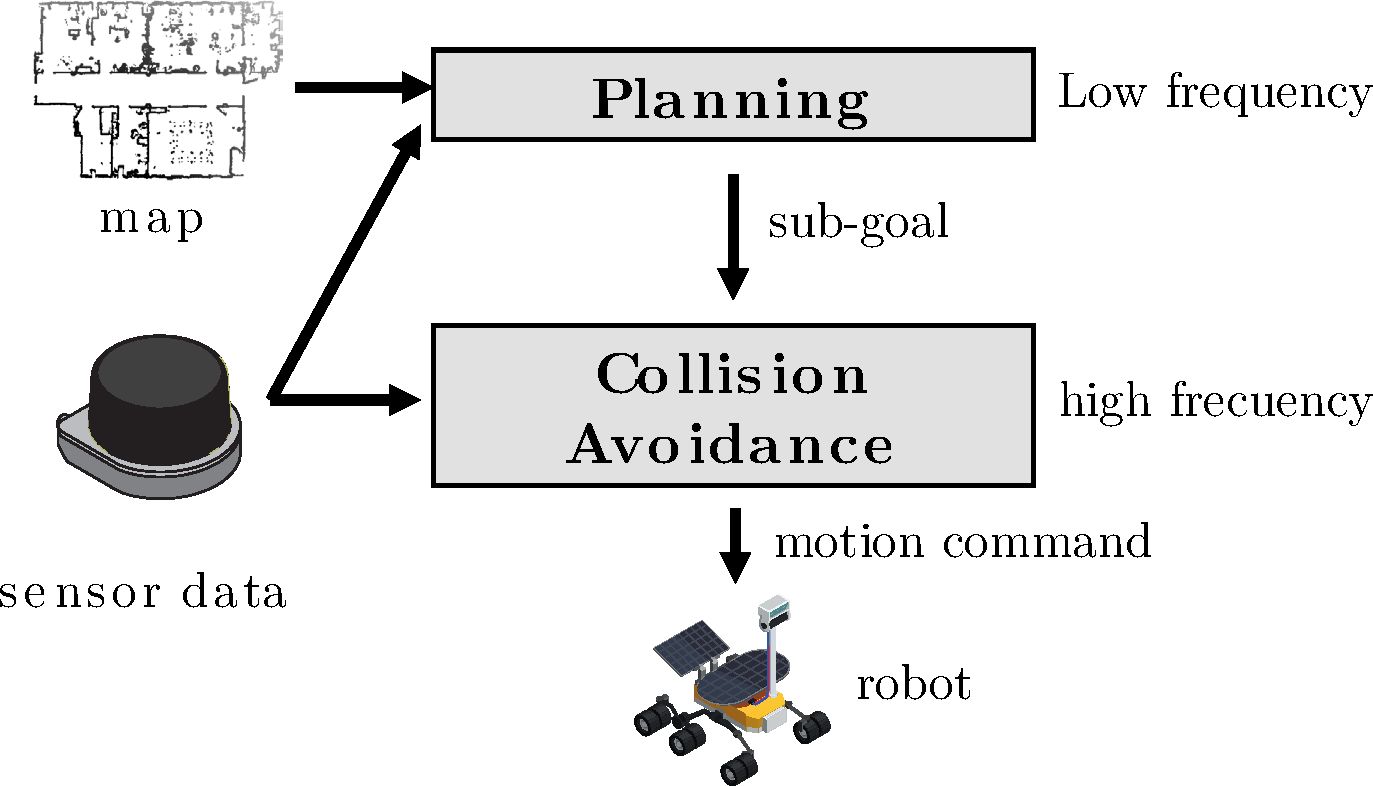
\includegraphics[width=0.8\textwidth]{images/path_planning_architecture.pdf}
	\end{figure}
    \note{El método de planning corre a baja frecuencia y genera sub-goals que los envía al método de Evasión de obstáculos. El método de evasión de obstáculos corre a alta frecuencia e intenta alcanzar los sub-goals. Mientras se dirige a un sub-goal evade obstáculos.}
	
\end{frame}

%\begin{frame}
%    \frametitle{Arquitectura clásica}
%    \note{Información extraída de slides de Martin Saska}
%    
%    \begin{figure}[!h]
%        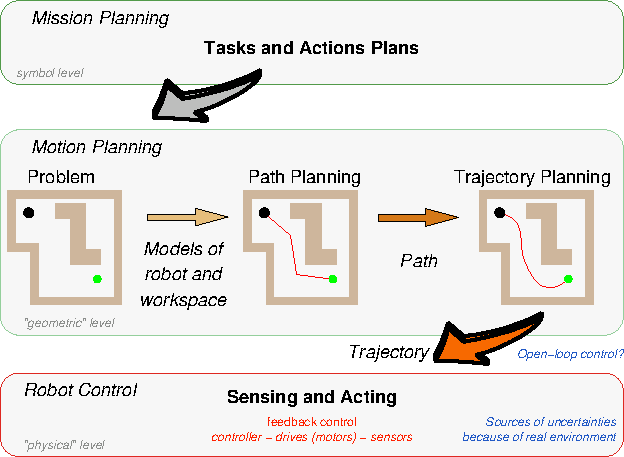
\includegraphics[width=0.6\textwidth]{images/motion_planning_architecture.pdf}
%    \end{figure}
%
%    {\bf Motion planning} es parte del ciclo de {\bf mission planning}. Los algoritmos offline se convierten en planificaciones online.
%    
%\end{frame}

\begin{frame}
    \frametitle{Formulación de Motion Planning}
    \note{Información extraída de http://ais.informatik.uni-freiburg.de/teaching/ss18/robotics/slides/19-pathplanning-long.pdf}
    
    \begin{itemize}
        \item El {\bf problema de la motion planning} se puede declarar de la siguiente manera. \textbf{Input:}
        \begin{itemize}
            \item Una \textbf{pose inicial} del robot
            \item Una \textbf{pose final} deseada
            \item Una \textbf{descripción geométrica del robot}
            \item Una \textbf{representación geométrica del entorno}
        \end{itemize}
        \item \textbf{Output:} Encontrar un camino que conduzca al robot desde el punto de inicio al punto final sin colisionar con los obstáculos
    \end{itemize}
\end{frame}

\begin{frame}
    \frametitle{Espacio de configuraciones}
    \note{Información extraída de Cyrill Stachniss - Robot Motion Planning using A*: https://youtu.be/HR1TNa8Lp7w}
    
    \begin{itemize}
        \item Aunque el problema de motion planning es definido en el mundo regular, vive en otro espacio: el {\bf Espacio de configuraciones} (lo notaremos con $\configurationSpace$)
        \item $\configurationSpace$-space: las posiciones de todos los puntos del robot en relación con un sistema de coordenadas fijo
        \item Una {\bf configuración de robot}, $\robotConfiguration$, es una especificación de las posiciones de todos los puntos del robot en relación con un sistema de coordenadas fijo
        \item Por lo general, el espacio de configuraciones es discretizado.
        \item Una configuración se expresa como un {\bf vector de posiciones y orientaciones}
    \end{itemize}
    
\end{frame}

\begin{frame}
    \frametitle{Espacio de configuraciones}
    \note{Información extraída de Cyrill Stachniss - Robot Motion Planning using A*: https://youtu.be/HR1TNa8Lp7w}
    
    \begin{itemize}
        \item Hay dos tipos de regiones: libres u ocupadas (con obstáculos)
        \item Sea $\workSpace = \mathbb{R}^{m}$ el \emph{work space} (para un mundo 2D, $\workSpace = \mathbb{R}^{2}$), $\obstaclesSet \in \workSpace$ el conjunto de obstáculos, un robot $\robotInConfiguration(\robotConfiguration)$ en la configuración $\robotConfiguration \in \configurationSpace$.
        La configuración del robot especifica completamente la pose del robot en $\workSpace$ incluyendo la especificación de todos los grados de libertad. (E.g., un robot con un cuerpo rígido en el plano $\configurationSpace = \begin{bmatrix}
            x & y & \theta
        \end{bmatrix} = \mathbb{R}^{2} \times S_{1}$ .)
        
        \begin{align*}
            \freeConfigurationSpace &= \left\lbrace \robotConfiguration \in \configurationSpace | \robotInConfiguration(\robotConfiguration) \cap \obstaclesSet =  \emptyset \right\rbrace\\
            \obstableConfigurationSpace &= \configurationSpace / \freeConfigurationSpace
        \end{align*}
        
        \item Definimos:\\
        $\startConfiguration$: configuración \emph{start}\\
        $\goalConfiguration$: configuración \emph{goal}
        
        
        \begin{tikzpicture}[remember picture,overlay]
            \node[xshift=-2.5cm,yshift=-2.5cm] at (current page.east) { 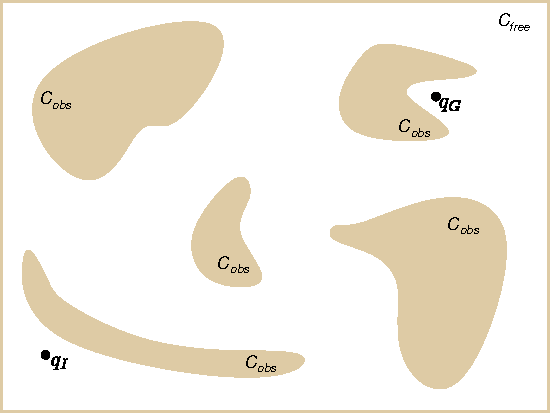
\includegraphics[height=0.4\textheight]{./images/configuration_space.pdf}};
        \end{tikzpicture}
       
    \end{itemize}
    
\end{frame}

%\begin{frame}
%    \frametitle{Ejemplo de espacio de configuraciones}
%    
%    \begin{figure}[!h]
%        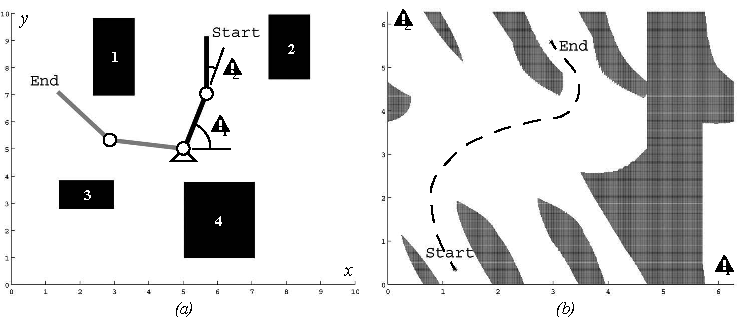
\includegraphics[width=0.8\textwidth]{images/configuration_space_manipulator.pdf}
%    \end{figure}
%    
%\end{frame}

\begin{frame}
    \frametitle{Espacio de Configuración}
    \note{Información extraída de Cyrill Stachniss - Robot Motion Planning using A*: https://youtu.be/HR1TNa8Lp7w}
    
    Entonces, Motion Planning equivale a 
    
    \begin{itemize}
        \item Encontrar un camino continuo
        \begin{equation*}
            \continuousPath : [0,1] \rightarrow \freeConfigurationSpace \quad \text{con} \quad \continuousPath(0) = \startConfiguration \quad \text{y} \quad  \continuousPath(1) = \goalConfiguration \quad \text{(\emph{solo hay consideraciones goemétricas})}
        \end{equation*} 
        \item Dada este seteo, podemos hacer planning con el robot siendo un punto en el $\configurationSpace$-space
    \end{itemize}

    \vspace{3em}

    \begin{tikzpicture}[remember picture,overlay]
        \node[xshift=-2.5cm,yshift=-2.5cm] at (current page.east) { 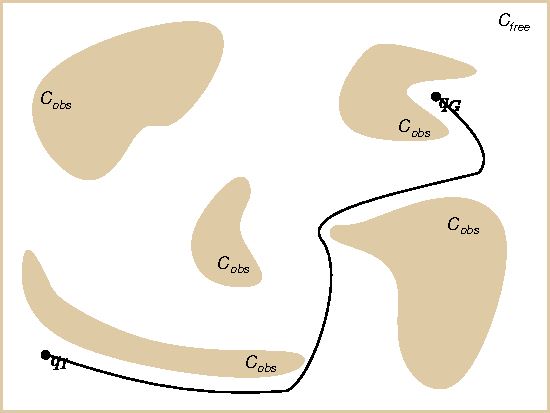
\includegraphics[height=0.4\textheight]{./images/configuration_space_with_path.pdf}};
    \end{tikzpicture}

\end{frame}

\begin{frame}
    \frametitle{Discretización del $\configurationSpace$-Space}
    \note{Información extraída de Cyrill Stachniss - Robot Motion Planning using A*: https://youtu.be/HR1TNa8Lp7w}
    
    \begin{itemize}
        \item El terreno continuo frecuentemente necesita ser discretizado para el planeamiento de de caminos
        \item Hay dos enfoques generales para discretizar $\configurationSpace$-spaces:
        \begin{itemize}
            \item \textbf{Combinatorial Planning}
            
            Caracteriza a $\configurationSpace$-space explícitamente capturando la conectividad del $\configurationSpace$-space en un grafo, y encuentra soluciones usando algoritmos de búsqueda
            
            \item \textbf{Sampling-based planning (Planificación basada en muestreo)}
            
            Utiliza detección de colisiones para sondear y buscar incrementalmente en el $\configurationSpace$-space una solución
        \end{itemize}

    \end{itemize}
    
    
    \TODO{Seguir las slides de Cyrill y luego con  \url{http://ais.informatik.uni-freiburg.de/teaching/ss18/robotics/slides/19-pathplanning-long.pdf} y Martín Saska}
    
\end{frame}

\begin{frame}
    \frametitle{Búsqueda}
    \note{Información extraída de Cyrill Stachniss - Robot Motion Planning using A*: https://youtu.be/HR1TNa8Lp7w}

    El problema de \textbf{búsqueda}: encontrar una secuencia de acciones (un camino, \emph{path}) que conduce a los estados deseable (una meta, \emph{goal})

    \begin{itemize}
        \item \textbf{Búsqueda desinformada:} además de la definición del problema, no hay más información sobre el dominio (\emph{blind search})
        \item Ampliar diferentes nodos con la esperanza de alcanzar el \emph{goal} en algún momento
        \item Ejemplos: breath-first, uniform-cost, depth-first, bidirectional, etc.
    \end{itemize}
       
\end{frame}


\begin{frame}
    \frametitle{Path vs Trajectory}
    \note{Información extraída de slides Martin Saska}
    
    \begin{itemize}
        \item {\bf Path}: es un mapeo continuo en $\configurationSpace$-space tal que
        \begin{equation*}
            \continuousPath : [0,1] \rightarrow \freeConfigurationSpace \quad \text{con} \quad \continuousPath(0) = \startConfiguration \quad \text{y} \quad  \continuousPath(1) = \goalConfiguration \quad \text{(\emph{solo hay consideraciones goemétricas})}
        \end{equation*} 
        \item {\bf Trajectory} es un camino con una parametrización explícita del movimiento del robot
        \begin{itemize}
            \item Ejemplo: acompañada por una descripción del las leyes de movimiento del robot
            \begin{equation*}
                \motionLaw : [0, 1] \rightarrow \robotActionSpace,
            \end{equation*}
            donde $\robotActionSpace$ es el espacio de acciones del robot. (\emph{incluye la dinámica del robot})
        \end{itemize}
        \vspace{3em}
        \begin{center}
            \alert{El problema de planeamiento consiste en determinar la función $\continuousPath(.)$}  
        \end{center}
    \end{itemize}
\end{frame}

\begin{frame}
    \frametitle{Problema de Motion Planning}
    \note{Información extraída de slides Martin Saska}
    
    \footnotesize
    
    Teniendo 
    \begin{itemize}
        \item La dinámica de un sistema con estado $\state$ y comandos de control $\controlCommand$
        \begin{equation*}
            \dfrac{\partial \state}{\partial t} = f(\state,\controlCommand)
        \end{equation*}
        \item Un conjunto de obstáculos $\obstaclesSet \subset \workSpace$ y un conjunto objetivo $\goalSet \subset \workSpace$     
    \end{itemize}
    El problema de Motion Planning consiste en encontrar el comando de control $\controlCommand$ tal que 
    \begin{equation*}
        \state(t) \notin \obstaclesSet \, \text{para} \,  t \in \mathbb{R}_{+} \, \text{y} \, \state(t) \in \goalSet \,  \forall t \ge T_{f} \, \text{para algún finito} \, T_{f} \geq 0,
    \end{equation*}    
    o, retorna que no existe tal señal de control.
    
    \begin{equation*}
        t \in [T_{0} , T_{f}] \rightarrow i \in [0, 1] : \robotConfiguration(t) = \continuousPath(i) \in \freeConfigurationSpace
    \end{equation*}
    
    Se pueden agregar requerimientos adicionales como
    \begin{itemize}
        \item Suavizado del camino
        \item Restricciones Kinodynamicas\footnote{La planificación kinodinámica se refiere a la tarea de conducir un robot desde un estado inicial hasta un estado objetivo mientras se evaden los obstáculos y se obedecen las restricciones cinemáticas y dinámicas (en resumen, kinodinámicas) que dictan la relación entre los controles del robot y su movimiento.} (\emph{e.g. considerando fuerzas de fricción})
        \item Criterio de Optimalidad (\emph{e.g. shortest vs fastest})
    \end{itemize}
\end{frame}


\begin{frame}
	\frametitle{Dynamic Window Approach}
	\note{Información extraída de http://ais.informatik.uni-freiburg.de/teaching/ss18/robotics/slides/19-pathplanning-long.pdf}
	
    \begin{itemize}
        \item \textbf{Evasión de obstáculos}: determine trayectorias libres de colisiones mediante operaciones geométricas
        \item El robot se mueve en arcos circulares, es decir utilizamos comandos de movimiento: $(v,\omega)$
        \item ¿Cuáles $(v,\omega)$ son admisibles y alcanzables?
    \end{itemize}
    
    \begin{center}
        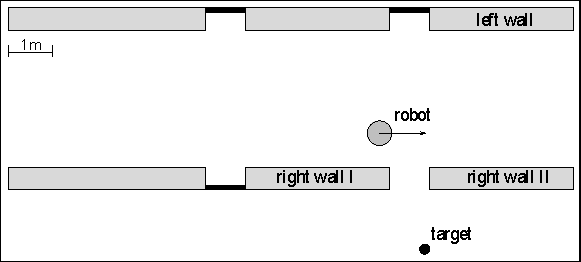
\includegraphics[width=0.6\columnwidth]{images/dynamic_window_approach_robot_world.pdf}
    \end{center}
    
\end{frame}

\begin{frame}
    \frametitle{Velocidades Admisibles}
    \note{Información extraída de http://ais.informatik.uni-freiburg.de/teaching/ss18/robotics/slides/19-pathplanning-long.pdf}
    
    \begin{itemize}
        \item Las velocidades son admisibles si el robot fuera capaz de detenerse antes de alcanzar un obstáculo
    \end{itemize}
    
    \begin{align*}
        V_{a} = \{ (v,\omega) \, | \,
              v &\leq \sqrt{2 dist(v,\omega) a_{trans}} \quad \land \\
         \omega &\leq \sqrt{2 dist(v,\omega) a_{rot}} \}
    \end{align*}
    
    \begin{center}
        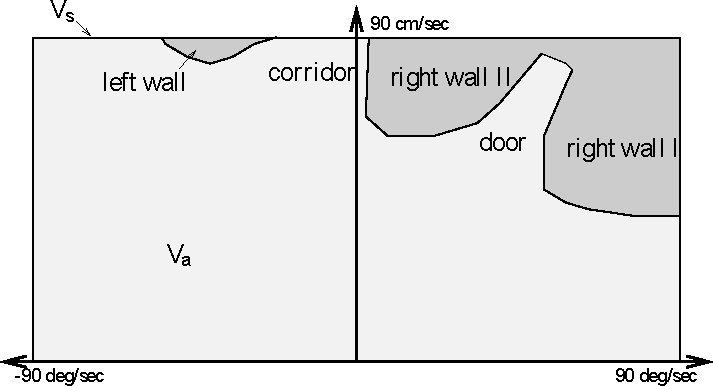
\includegraphics[width=0.6\columnwidth]{images/dynamic_window_approach_admissible_velocities.pdf}
    \end{center}
    
\end{frame}

\begin{frame}
    \frametitle{Velocidades Alcanzables}
    \note{Información extraída de http://ais.informatik.uni-freiburg.de/teaching/ss18/robotics/slides/19-pathplanning-long.pdf}
    
    \begin{align*}
        V_{a} = \{ (v,\omega) \, | \,
        v &\in \left[ v - a_{trans} t, v + a_{trans} t \right] \quad \land \\
        \omega &\in \left[ \omega - a_{rot} t, \omega + a_{rot} t \right] \}
    \end{align*}
    
    \begin{center}
        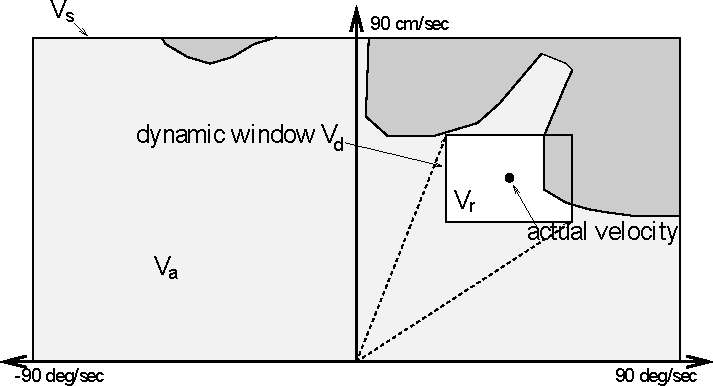
\includegraphics[width=0.7\columnwidth]{images/dynamic_window_approach_recheable_velocities.pdf}
    \end{center}
    
\end{frame}

\begin{frame}
    \frametitle{DWA Espacio de Búsqueda}
    \note{Información extraída de http://ais.informatik.uni-freiburg.de/teaching/ss18/robotics/slides/19-pathplanning-long.pdf}
    
    \begin{center}
        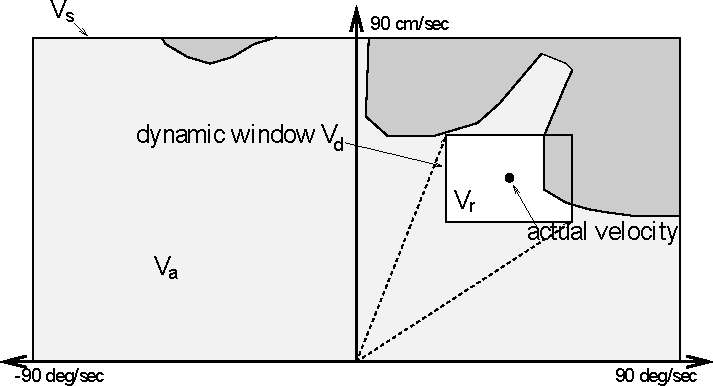
\includegraphics[width=0.7\columnwidth]{images/dynamic_window_approach_recheable_velocities.pdf}
    \end{center}
    
    
    \TODO{Completar con slides: \url{http://ais.informatik.uni-freiburg.de/teaching/ss18/robotics/slides/19-pathplanning-long.pdf}}
\end{frame}

\begin{frame}
    \frametitle{Dynamic Window Approach}
    \note{Información extraída de http://ais.informatik.uni-freiburg.de/teaching/ss18/robotics/slides/19-pathplanning-long.pdf}
    
    
    \TODO{Completar con slides: \url{http://ais.informatik.uni-freiburg.de/teaching/ss18/robotics/slides/19-pathplanning-long.pdf}}
    
    
\end{frame}

\begin{frame}
    \frametitle{Dynamic Window Approach}
    \note{Información extraída de http://ais.informatik.uni-freiburg.de/teaching/ss18/robotics/slides/19-pathplanning-long.pdf}
    
    
    \TODO{Completar con slides: \url{http://ais.informatik.uni-freiburg.de/teaching/ss18/robotics/slides/19-pathplanning-long.pdf}}
    
    
\end{frame}

\begin{frame}
    \frametitle{Dynamic Window Approach}
    \note{Información extraída de http://ais.informatik.uni-freiburg.de/teaching/ss18/robotics/slides/19-pathplanning-long.pdf}
    
    
    \TODO{Completar con slides: \url{http://ais.informatik.uni-freiburg.de/teaching/ss18/robotics/slides/19-pathplanning-long.pdf}}
    
    
\end{frame}

\begin{frame}
    \frametitle{Dynamic Window Approach}
    \note{Información extraída de http://ais.informatik.uni-freiburg.de/teaching/ss18/robotics/slides/19-pathplanning-long.pdf}
    
    
    \TODO{Completar con slides: \url{http://ais.informatik.uni-freiburg.de/teaching/ss18/robotics/slides/19-pathplanning-long.pdf}}
    
    
\end{frame}

%\begin{frame}
%	\frametitle{Espacio de configuraciones}
%
%	%Espacio de configuraciones es el estado total del robot y el entorno, incluidas las articulaciones y/o movimiento de ruedas)
%	
%	\begin{figure}[!h]
	%		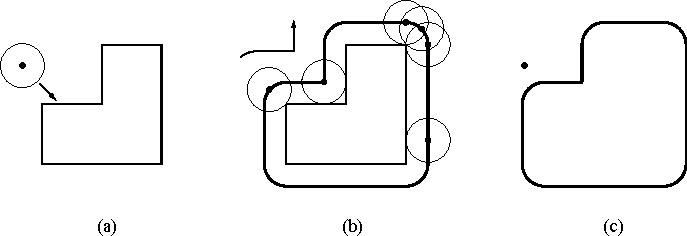
\includegraphics[width=0.8\textwidth]{images/configuration_space_obstacle.pdf}
	%	\end{figure}
%	
%\end{frame}
%
%\begin{frame}
%	\frametitle{Espacio de configuraciones}
%	
%	\begin{figure}[!h]
	%		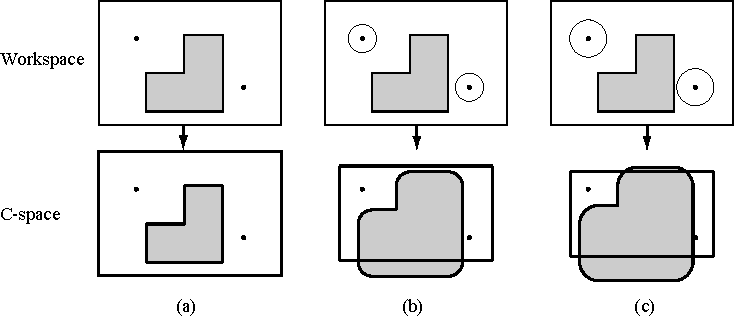
\includegraphics[width=0.8\textwidth]{images/workspace_configuration_space.pdf}
	%	\end{figure}
%	
%\end{frame}
%
%
%\begin{frame}
%    \frametitle{Espacio de configuraciones}
%    \note{Información extraída de slides Martin Saska}
%    
%    \begin{figure}[!h]
	%        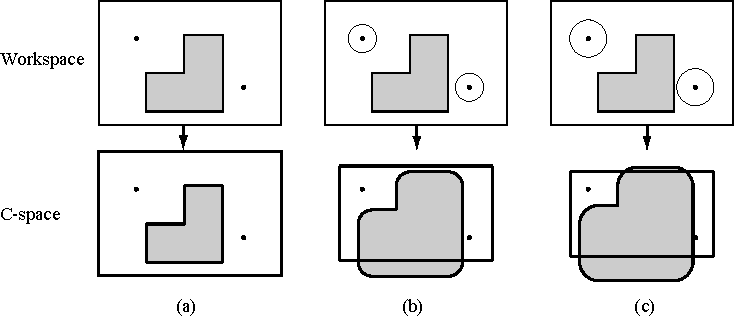
\includegraphics[width=0.8\textwidth]{images/workspace_configuration_space.pdf}
	%    \end{figure}
%    
%\end{frame}

\begin{frame}
	\frametitle{Ejemplo de planeamiento sencillo en el $\configurationSpace$-space}
	\note{Información extraída de slides Martin Saska}
	
	\begin{figure}
		\subfloat[Problema Motion planning en representación geométrica de $\workSpace$]
		{
			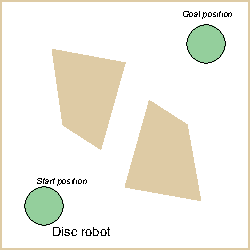
\includegraphics[width=0.33\textwidth]{images/motion_planning_geometrical_example.pdf}
		}\hspace{1em}
		\subfloat[Problema de Motion planning en representación $\configurationSpace$-space]
		{
			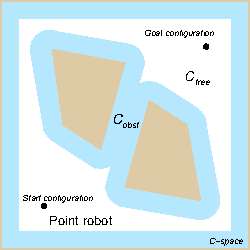
\includegraphics[width=0.33\textwidth]{images/motion_planning_cspace_example.pdf}
		}
	\end{figure}
	
En este ejemplo, $\configurationSpace$-space es obtenido por medio de agrandar los obstáculos por el disco $\robotActionSpace$ con radio $\rho$. Aplicando la suma de Minkowski: $\obstaclesSet + \robotActionSpace = \{ x \oplus y | x \in \obstaclesSet, y \in \robotActionSpace \}$
	
\end{frame}

\begin{frame}
	\frametitle{Ejemplo $\obstableConfigurationSpace$ para un robot con rotación}
	\note{Información extraída de slides Martin Saska}
	
	\begin{figure}[!h]
		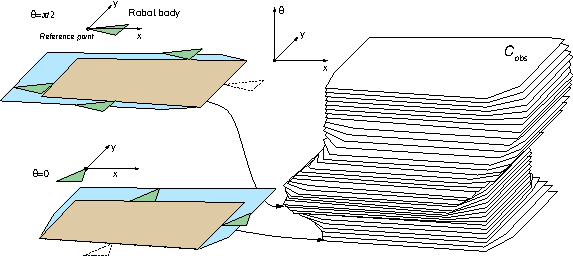
\includegraphics[width=0.6\textwidth]{images/cspace_representation_motivation.pdf}
		\caption{Un simple obstáculo 2D tiene un complicado $\obstableConfigurationSpace$}
	\end{figure}

	\begin{itemize}
		\item Existe un algoritmo determinístico\footnote{J. Canny, PAMI, 8(2):200–209, 1986} pero requiere tiempo exponencial en el número de dimensiones de $\configurationSpace$
		\item Una representación explícita de $\freeConfigurationSpace$ en computacionalmente intratable.
	\end{itemize}
\end{frame}

\begin{frame}
	\frametitle{Representación de $\configurationSpace$-space}
	\note{Información extraída de slides Martin Saska}
	
	¿Cómo podemos lidiar con una representación continua de $\configurationSpace$-space?
	
	\begin{figure}[!h]
		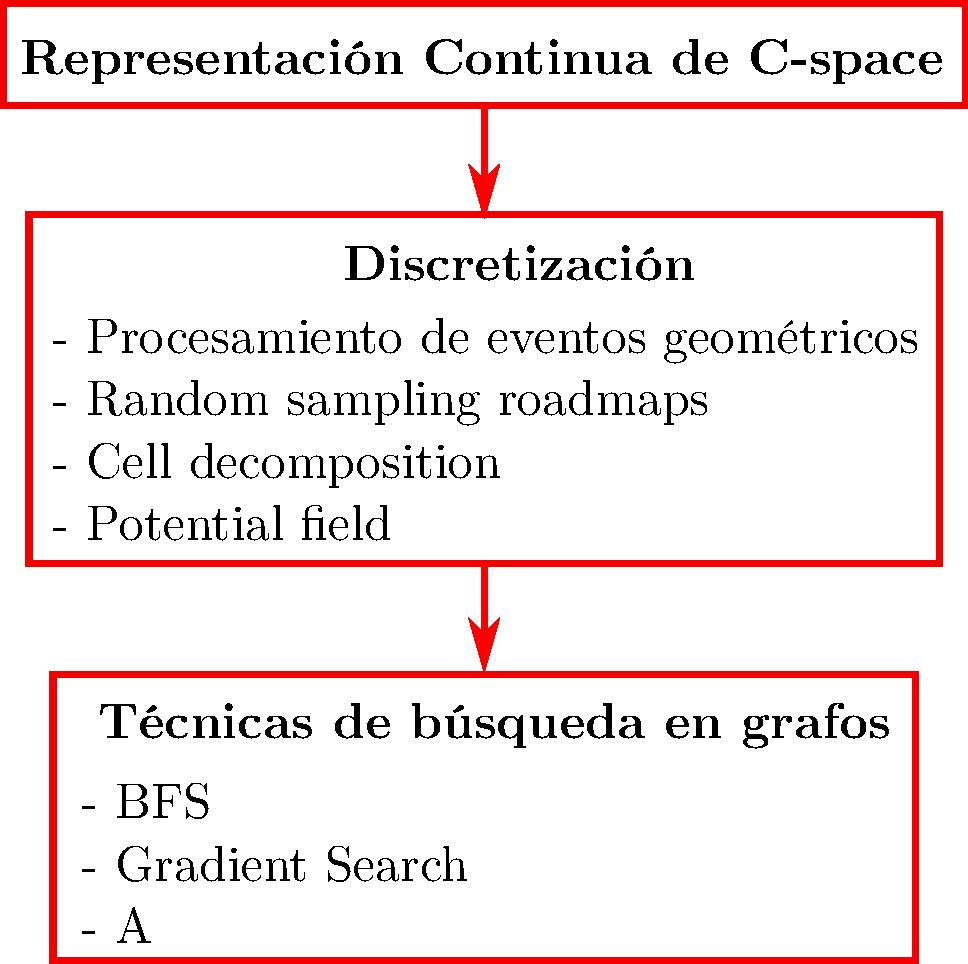
\includegraphics[width=0.4\textwidth]{images/cspace_representation.pdf}
	\end{figure}
	
\end{frame}


\begin{frame}
	\frametitle{Métodos de planning}
	\note{Información extraída de slides Martin Saska}
	
	{\bf Algoritmos clásicos de Planeamiento de caminos}
	
	\begin{itemize}
		\item Métodos basados en Roadmap (crear un grafo de conectividad del espacio libre)
		\begin{itemize}
			\item Visibility graph
			\item Cell decomposition
			\item Voronoi diagram
		\end{itemize}
		\item Métodos basados en Potential field
	\end{itemize}

	{\bf Randomized path/motion planning approaches}
	\begin{itemize}
		\item Probabilistic roadmaps (PRM)
		\item Expansive-Spaces Tree (EST)
		\item Rapidly-Exploring Random Tree (RRT) $\leftarrow$ Permite considerar restricciones kinodinámicas.
		\item Optimal sampling based Planner - RRT*
	\end{itemize}
\end{frame}

\begin{frame}
	\frametitle{Visibility Graph}
	\note{Información extraída de slides Martin Saska}
	
	\begin{enumerate}
		\item Computar el visibility graph
		\item Encontrar el camino más corto (e.g. utilizando el algoritmo de Dijkstra)
	\end{enumerate}
	
	\begin{figure}
		\subfloat[Problem]
		{
			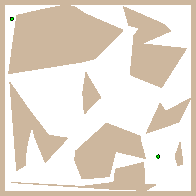
\includegraphics[width=0.2\textwidth]{images/visibility_graph_problem.pdf}
		}\hspace{1em}
		\subfloat[Visibility graph]
		{
			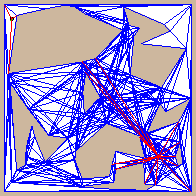
\includegraphics[width=0.2\textwidth]{images/visibility_graph.pdf}
		}\hspace{1em}
		\subfloat[Camino más corto encontrado]
		{
			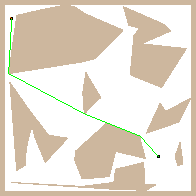
\includegraphics[width=0.2\textwidth]{images/visibility_graph_path.pdf}
		}
	\end{figure}

	Construcción del visibility graph:
	\begin{enumerate}
		\item Naïve -- todos los segmentos entre $n$ vértices del mapa $O(n^{3})$
		\item Utilizar árboles de rotación\footnote{M. H. Overmars and E. Welzl, 1988} para un conjunto de segmentos $O(n^{2})$
	\end{enumerate}
	
\end{frame}

\begin{frame}
	\frametitle{Voronoi Diagram}
	\note{Información extraída de slides Martin Saska}
	
	\begin{enumerate}
		\item El roadmap es un diagrama de Voronoi que {\bf maximiza el espacio libre} entre los obstáculos
		\item Las posiciones de inicio y meta se conectan al grafo
		\item La ruta se encuentra usando un algoritmo de búsqueda de grafos
	\end{enumerate}
	
	\begin{figure}
		\subfloat[Voronoi diagram]
		{
			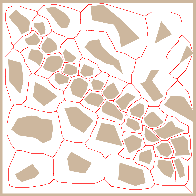
\includegraphics[width=0.2\textwidth]{images/voronoi_diagram_problem.pdf}
		}\hspace{1em}
		\subfloat[Camino en el grafo]
		{
			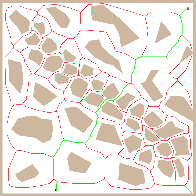
\includegraphics[width=0.2\textwidth]{images/voronoi_diagram.pdf}
		}\hspace{1em}
		\subfloat[Camino encontrado]
		{
			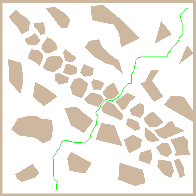
\includegraphics[width=0.2\textwidth]{images/voronoi_diagram_path.pdf}
		}
	\end{figure}
	
\end{frame}


\begin{frame}
	\frametitle{Visibility Graph vs Voronoi Diagram}
	\note{Información extraída de slides Martin Saska}
	
	\TODO{Completar con slides ECI2015 Martín Saska}
	
\end{frame}

\begin{frame}
	\frametitle{Visibility - Voronoi complex}
	\note{Información extraída de slides Martin Saska}
	
	\TODO{Completar con slides ECI2015 Martín Saska}
	
\end{frame}


\begin{frame}
	\frametitle{Cell Decomposition}
	\note{Información extraída de slides Martin Saska}
	
	\begin{enumerate}
		\item Descomponer el espacio libre en partes. Dos puntos cualesquiera en una región convexa pueden estar directamente conectado por un segmento.
		\item Crear un grafo de adyacencia que represente la conectividad del espacio libre.
		\item Encuentra un camino en el grafo.
	\end{enumerate}
	
	\begin{figure}
		\subfloat[Los centroides reprensetan celdas]
		{
			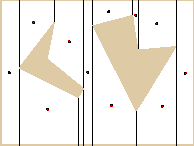
\includegraphics[width=0.2\textwidth]{images/cell_decomposition_centroids.pdf}
		}\hspace{1em}
		\subfloat[Conectar celdas adyacentes]
		{
			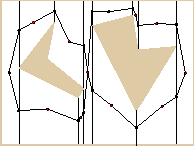
\includegraphics[width=0.2\textwidth]{images/cell_decomposition_adjacency_cells.pdf}
		}\hspace{1em}
		\subfloat[Encontrar el camino en el grafo de adyacencia]
		{
			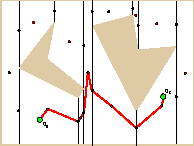
\includegraphics[width=0.2\textwidth]{images/cell_decomposition_path.pdf}
		}
	\end{figure}
	
\end{frame}

\begin{frame}
	\frametitle{Global Planner vs Local Planner}
	
	\begin{figure}[!h]
		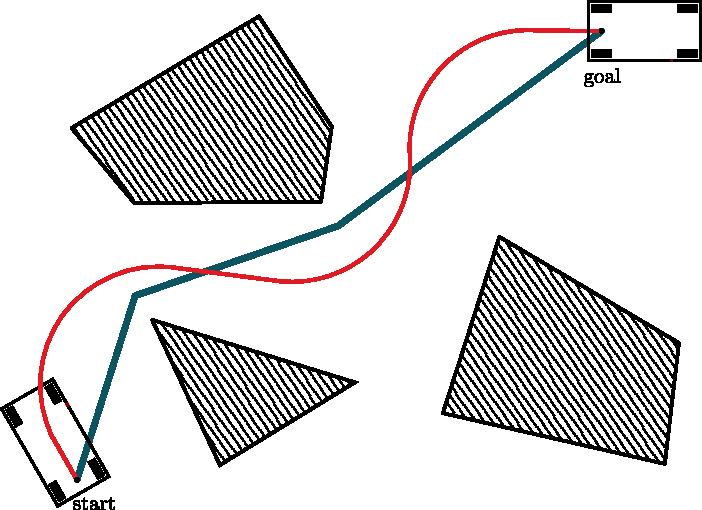
\includegraphics[width=0.5\textwidth]{images/global_local_plan.pdf}
	\end{figure}
	
\end{frame}

\begin{frame}
	\frametitle{Potential Field}
	
	\begin{figure}
		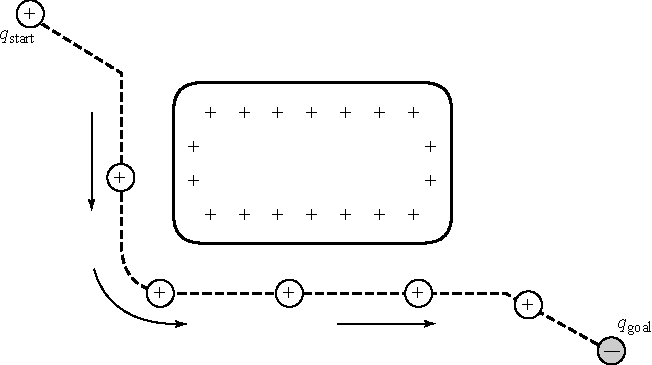
\includegraphics[width=0.6\textwidth]{images/potential_field_concept.pdf}
	\end{figure}
	
\end{frame}

\begin{frame}
	\frametitle{Potential Field}
	\note{Información extraída de slides Martin Saska}
	
	\begin{figure}
	\subfloat[]
	{
		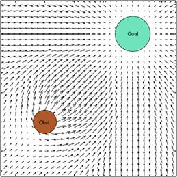
\includegraphics[width=0.25\textwidth]{images/potential_field_example.pdf}
	}\hfill
	\subfloat[]
	{
		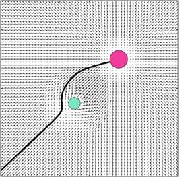
\includegraphics[width=0.25\textwidth]{images/potential_field_path_example.pdf}
	}\hfill
	\subfloat[]
	{
		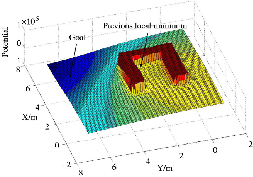
\includegraphics[width=0.4\textwidth]{images/potential_field_3d_representation.pdf}
	}
	\end{figure}

\end{frame}

\begin{frame}
	\frametitle{Local Path Planning - Bug1}
	\note{Información extraída de slides Martin Saska}
	
	\begin{itemize}
		\item Rodear el obstáculo para esquivarlo
		\item Cada obstáculo encontrado se rodea completamente una vez, antes de que sea
		dejado en el punto más cercano a la meta
		\item No retorna un camino óptimo; funciona bien con pequeños obstáculos convexos
	\end{itemize}
	
	\begin{figure}
		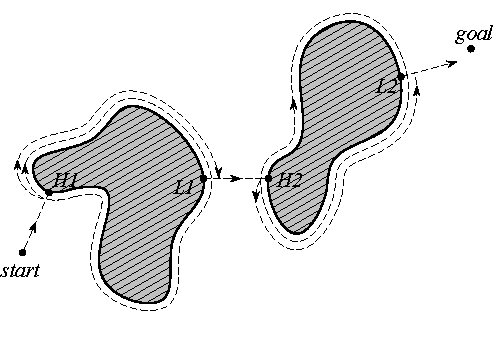
\includegraphics[width=0.6\textwidth]{images/bug1.pdf}
	\end{figure}
\end{frame}

\begin{frame}
	\frametitle{Local Path Planning - Bug2}
	\note{Información extraída de slides Martin Saska}
	
	\begin{itemize}
		\item Rodear el obstáculo siempre por el lado izquierdo o derecho
		\item Dejar el obstáculo si la conexión directa entre inicio y meta se cruzan
	\end{itemize}
	
	\begin{figure}
		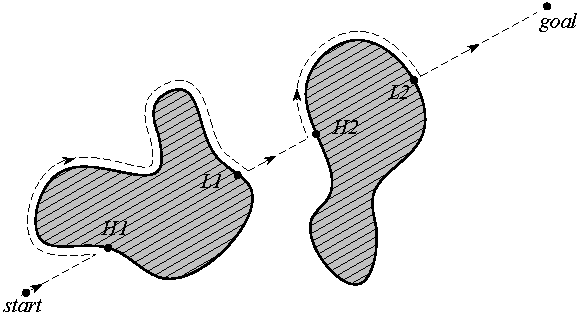
\includegraphics[width=0.7\textwidth]{images/bug2.pdf}
	\end{figure}
	
\end{frame}

\begin{frame}
	\frametitle{Local Path Planning - Vector Field Histogram (VFH)}
	\note{Información extraída de slides Martin Saska}
	
	\begin{itemize}
		\item Rayo láser virtual en 360 grados
		\item Obtenido por sensor range-finder
		\item Se selecciona la dirección con la función de menor costo $G$
	\end{itemize}

	\begin{equation*}
		G = a.targetDirection + b.wheelOrientation + c.previousDirection
	\end{equation*}
	
	\begin{figure}
		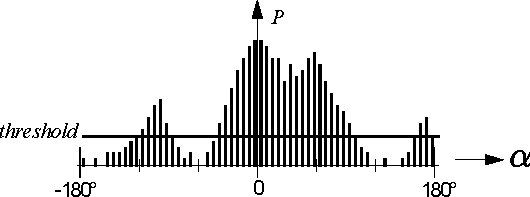
\includegraphics[width=0.7\textwidth]{images/obstacle_avoidande_plor_histogram.pdf}
	\end{figure}
	
\end{frame}

\begin{frame}
	\frametitle{Local Path Planning - Vector Field Histogram+ (VFH+)}
	\note{Información extraída de slides Martin Saska}
	
	\begin{itemize}
		\item E.g. para robot car-like
		\item Considera las restricciones de movimiento cinemático de los robots
		\item Es necesaria la construcción de un mapa local
	\end{itemize}
	
	\begin{figure}
		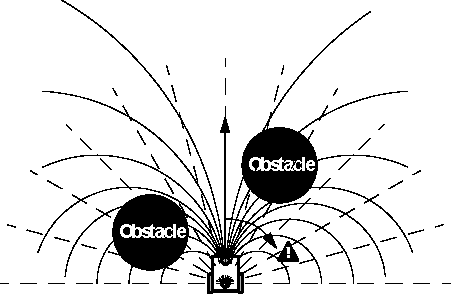
\includegraphics[width=0.5\textwidth]{images/vfh_plus.pdf}
	\end{figure}
	
\end{frame}

\begin{frame}
	\frametitle{Sampling-based Motion Planning}
	\note{Información extraída de slides Martin Saska}
	
	\begin{itemize}
		\item Evita la representación explícita de obstáculos en el $\configurationSpace$-space
        \item Se utiliza una función de ``caja negra'' para evaluar una configuración $\robotConfiguration$
		es libre de colisiones (Por ejemplo, basado en modelos geométricos y pruebas
		colisiones de los modelos)
		\item Crea una representación discreta de $\freeConfigurationSpace$
		\item Las configuraciones en $\freeConfigurationSpace$ se muestrean aleatoriamente y se conectan
		a una roadmap (Probabilistic roadmap)
		\item En lugar de una completa exhaustividad, proporcionan datos probabilísticos completitud o resolución completitud. Algoritmos probabilísticos completos: con un número creciente de muestras se encontraría una solución admisible (si existe)
	\end{itemize}
	
\end{frame}

\begin{frame}
	\frametitle{Probabilistic Roadmap}
	\note{Información extraída de slides Martin Saska}
	
	Una representación discreta del espacio C continuo generado
	por configuraciones muestreadas aleatoriamente en Cfree que están conectadas
	en un gráfico.
	\begin{itemize}
		\item Los {\bf nodos} del grafo representan la configuración admisible de
		el robot.
		\item Las {\bf aristas} representan un camino factible (trayectoria) entre el
		configuraciones particulares.
	\end{itemize}

	Teniendo el grafo, la ruta final (trayectoria) se encuentra mediante una técnica de búsqueda de grafos.
\end{frame}

\begin{frame}
	\frametitle{Probabilistic Roadmap Strategies}
	\note{Información extraída de slides Martin Saska}
	
	{\bf Multi-Query (Batch)}:
	\begin{itemize}
	\item Generar un único roadmap (mapa de rutas) que luego se utiliza para planificar varias veces.
		\begin{itemize}
			\item Probabilistic RoadMap – PRM
		\end{itemize}
	\end{itemize}

	{\bf Single-Query (Incremental)}:
	\begin{itemize}
		\item Para cada problema de planificación se construye un nuevo roadmap para
		caracterizar el subespacio del $\configurationSpace$-space que es relevante.
		\begin{itemize}
			\item Rapidly-exploring Random Tree -- RRT\footnote{LaValle, 1998}
			\item Expansive-Space Tree -- EST\footnote{Hsu et al., 1997}
			\item Sampling-based Roadmap of Trees – SRT\footnote{Plaku et al., 2005}
		\end{itemize}
	\end{itemize}

\end{frame}

\begin{frame}
	\frametitle{Probabilistic RoadMap (PRM) Planner}
	\note{Información extraída de slides Martin Saska}
	
	Construir una roadman (grafo) que represente el entorno
	\begin{itemize}
		\item Etapa de aprendizaje
		\begin{enumerate}
			\item Muestrar $n$ puntos en $\freeConfigurationSpace$
			\item Conectar las configuraciones aleatorias usando un local planner
		\end{enumerate}
		\item Etapa de consulta
		\begin{enumerate}
			\item Conectar las configuraciones de inicio y meta con el PRM. Por ejemplo, usando un local planner
			\item Usar la búsqueda grafo para encontrar la ruta
		\end{enumerate}
	\end{itemize}
\end{frame}

\begin{frame}
	\frametitle{PRM Construction/Query}
	\note{Información extraída de slides Martin Saska}
	

	\only<1>{
		\begin{figure}[!h]
			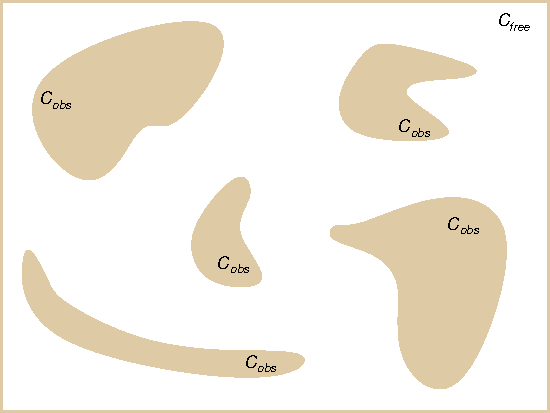
\includegraphics[width=0.6\textwidth]{images/prm_problem.pdf}
			\caption{Domino del problema}
		\end{figure}
	}
	\only<2>{
		\begin{figure}[!h]
			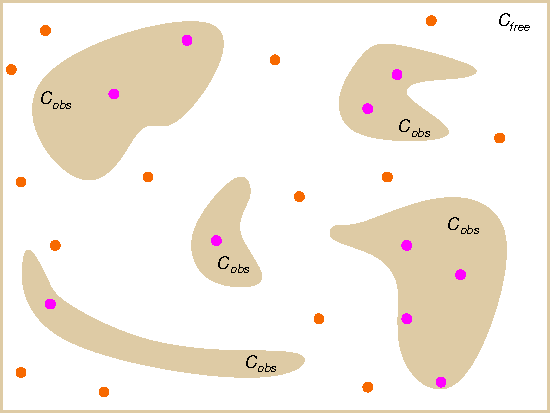
\includegraphics[width=0.6\textwidth]{images/prm_random_configurations.pdf}
			\caption{Configuraciones aleatorias}
		\end{figure}
	}
	\only<3>{
		\begin{figure}[!h]
			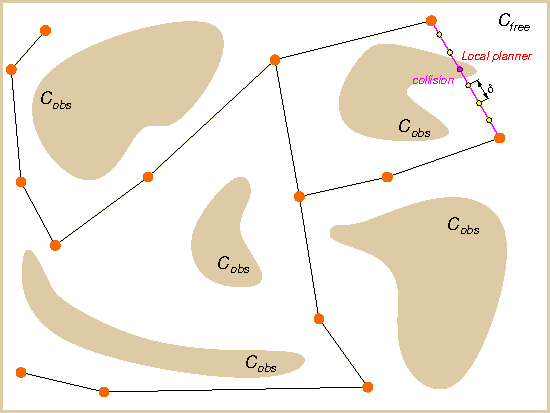
\includegraphics[width=0.6\textwidth]{images/prm_connect_random_samples.pdf}
			\caption{Conectando configuraciones aleatorias}
		\end{figure}
	}
	\only<4>{
		\begin{figure}[!h]
			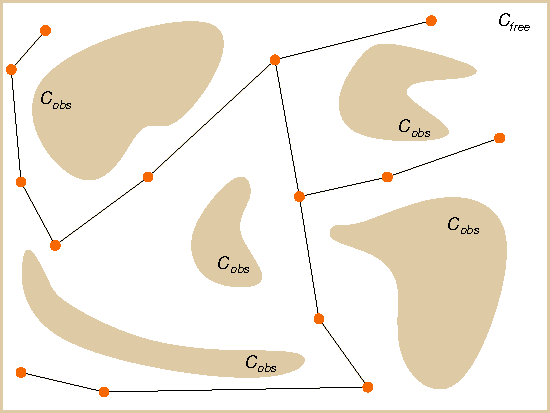
\includegraphics[width=0.6\textwidth]{images/prm_connected_roadmap.pdf}
			\caption{Ruta conectada}
		\end{figure}
	}
	\only<5>{
		\begin{figure}[!h]
			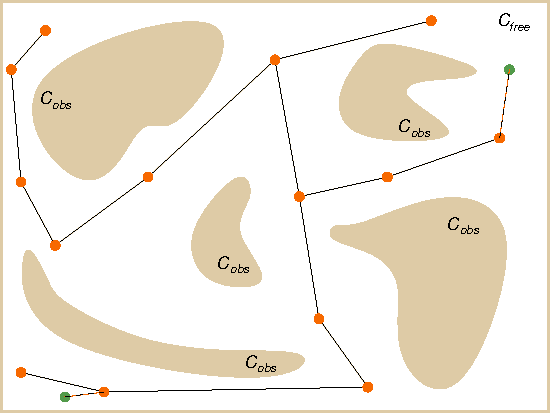
\includegraphics[width=0.6\textwidth]{images/prm_query_configuration.pdf}
			\caption{Consultar configuraciones}
		\end{figure}
	}
	\only<6>{
		\begin{figure}[!h]
			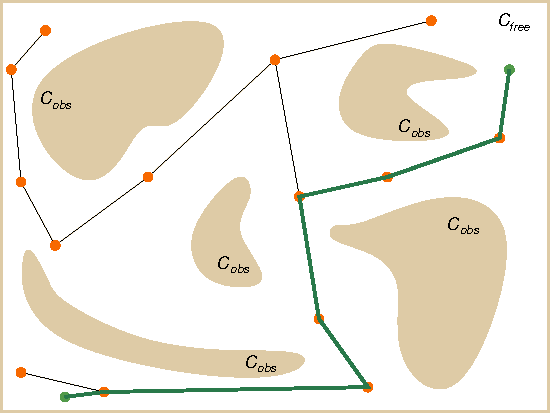
\includegraphics[width=0.6\textwidth]{images/prm_find_final_path.pdf}
			\caption{Encontrar el camino final}
		\end{figure}
	}
	
\end{frame}


\begin{frame}
	\frametitle{PRM - Resumen}
	\note{Información extraída de slides Martin Saska}
	
	\begin{columns}
		\begin{column}{0.5\textwidth}
			\begin{itemize}
				\item Construcción incremental
				\item Conectar nodos en un radio $\rho$
				\item El local planner prueba las colisiones hasta la resolución seleccionada $\delta$
				\item La ruta se puede encontrar mediante el algoritmo de Dijkstra
			\end{itemize}
		\end{column}
		\begin{column}{0.5\textwidth}  %%<--- here
			\begin{figure}[!h]
				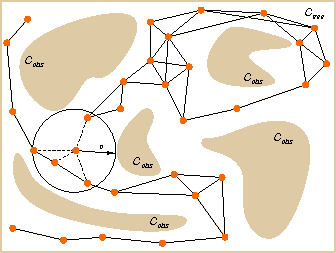
\includegraphics[width=\columnwidth]{images/prm_summary.pdf}
			\end{figure}
		\end{column}
	\end{columns}
	
\end{frame}

\begin{frame}
	\frametitle{Rapidly-exploring Random Trees (RRTs)}
	\note{Información extraída de slides Martin Saska}
	
	\begin{itemize}
		\item La motivación es una única consulta y una búsqueda de ruta basada en el control
		\item Construye incrementalmente un grafo (árbol) hacia el área objetivo.
	\end{itemize}
	
\end{frame}

\begin{frame}
	\frametitle{Rapidly-exploring Random Trees (RRTs)}
	\note{Información extraída de slides Martin Saska}
	
	\begin{figure}
		\subfloat[1. Nueva configuración aleatoria]
		{
			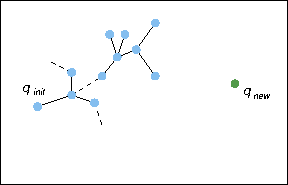
\includegraphics[width=0.25\textwidth]{images/rrt_construction1.pdf}
		}\hspace{1em}
		\subfloat[2. Seleccionar el nodo más cercano]
		{
			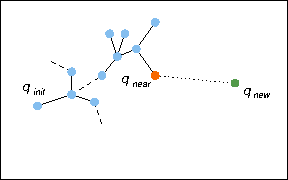
\includegraphics[width=0.25\textwidth]{images/rrt_construction2.pdf}
		}\\
		\subfloat[3. Posibles acciones desde $\robotConfiguration_{near}$]
		{
			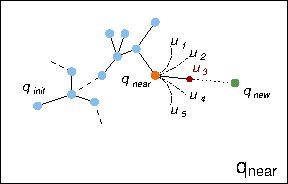
\includegraphics[width=0.25\textwidth]{images/rrt_construction3.pdf}
		}\hspace{1em}
		\subfloat[4. Extender el árbol]
		{
			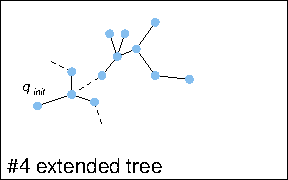
\includegraphics[width=0.25\textwidth]{images/rrt_construction4.pdf}
		}\\
	\end{figure}

	La expansión se repite hasta que se alcanza el $\goalConfiguration$ o la iteración máxima.

\end{frame}


\begin{frame}
	\frametitle{Propiedades de los algoritmos RRTs}
	\note{Información extraída de slides Martin Saska}

	\begin{itemize}
		\item Explora rápidamente el espacio qnew probablemente se generará en zonas grandes todavía no cubiertas de $\freeConfigurationSpace$.
		\item Permite considerar restricciones cinemáticas/dinámicas durante la expansión
		\item Puede proporcionar una trayectoria o una secuencia de comandos de control directo.
		\item Una prueba de detección de colisiones generalmente se usa como una ``caja negra''. Por ejemplo, las librerías RAPID, Bullet.
		\item Rendimiento deficiente en problemas de paso angosto similar a PRM
		\item Proporciona caminos factibles (más expansiones pueden mejorar los caminos)
		\item Se han propuesto muchas variantes de RRT
	\end{itemize}
\end{frame}

\begin{frame}
    \frametitle{Car-Like Robot}
    \note{Información extraída de slides Martin Saska}
    
    \TODO{Completar con slides ECI2015 Martín Saska}
    
\end{frame}

\begin{frame}
	\frametitle{Sampleo basado en control}
	\note{Información extraída de slides Martin Saska}
	
	\begin{figure}
		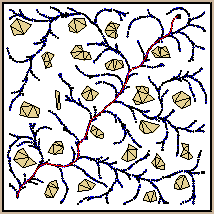
\includegraphics[width=0.5\textwidth]{images/rrt_control_based_sampling.pdf}
	\end{figure}
\end{frame}

